\documentclass[10pt]{beamer}
\usepackage{graphicx}
\usetheme{Madrid}

\begin{document}

\title{l'évolution des ordinateurs dans le temps}
\author{Ludwig AUREL, Anass TALEB, Ibrahima TRAORE, Rodrigue YOBA SALOMON}
\institute{TARL}
\date{24/11/2023}
\maketitle

\begin{frame}

	\frametitle{Sommaire}
	
	\begin{enumerate}
		\item Introduction
		\item Définition 
		\item Les Premiers Ordinateurs (machines à calculer)
		\item Les machines avec des circuits éléctriques
		\item Les premiers ordinateurs personnels
		\item Conclusion
	\end{enumerate}
	
\end{frame}

\begin{frame}

	\frametitle{Introduction}
	
	\begin{itemize}
		\item Prennent une place de plus en plus importante.
		\item Evolution rapide de celles-ci.
		\item La manière compte également.
	\end{itemize}
	
	\begin{alertblock}{Attention}
	L'informatique et l'ordinateur sont deux notions différentes.
	\end{alertblock}
	
\end{frame}

\begin{frame}

	\frametitle{Définition}
	
	\begin{itemize}
		\item Terme crée en 1955 par Jacques Perret.
		\item Rien à voir avec une traduction littérale de "computer".
		\item Recherche de l'efficacité.
	\end{itemize}
	
	\begin{flushright}
		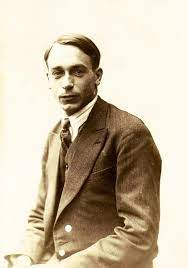
\includegraphics[width=0.3\textwidth]{Images/Jacques_Perret.jpg}
	\end{flushright}


\end{frame}


\begin{frame}[t]

	\frametitle{Les premiers ordinateurs (machines à calculer) : Le Boulier}

	\begin{itemize}
		\item Un des premiers ordinateurs crée au 7è siècle avant J.C.
		\item Permet de faire des calculs de façon manuelle.
		\item Encore utilisé aujourd'hui en Chine et en Russie.
	\end{itemize}
	
		\begin{center}
			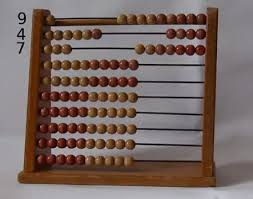
\includegraphics[width=0.5\textwidth]{Images/Boulier.jpg}
		\end{center}

\end{frame}

\begin{frame}[t]

	\frametitle{Les premiers ordinateurs (machines à calculer) : La Pascaline}
	
	\begin{itemize}
		\item Créée par Blaise Pascal en 1642.
		\item Permet d'effectuer des additions et des soustractions de façon automatique.
		\item Invention révolutionnaire
	\end{itemize}
	
			\begin{center}
				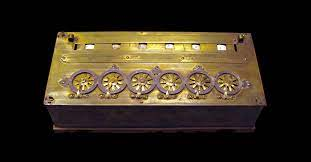
\includegraphics[width=0.5\textwidth]{Images/Pascaline2.jpg}
			\end{center}

\end{frame}

\begin{frame}[t]

	\frametitle{Les machines avec des circuits éléctriques : le Z3}
		
	\begin{itemize}
		\item Premier ordinateur programmable et éléctromécanique de l'histoire.
		\item Crée en 1941 pendant la 2nde Guerre Mondiale.
		\item Capable de traiter des nombres décimaux.
		\item Beaucoup utilisée dans le génie civil.
	\end{itemize}
	
			\begin{center}
				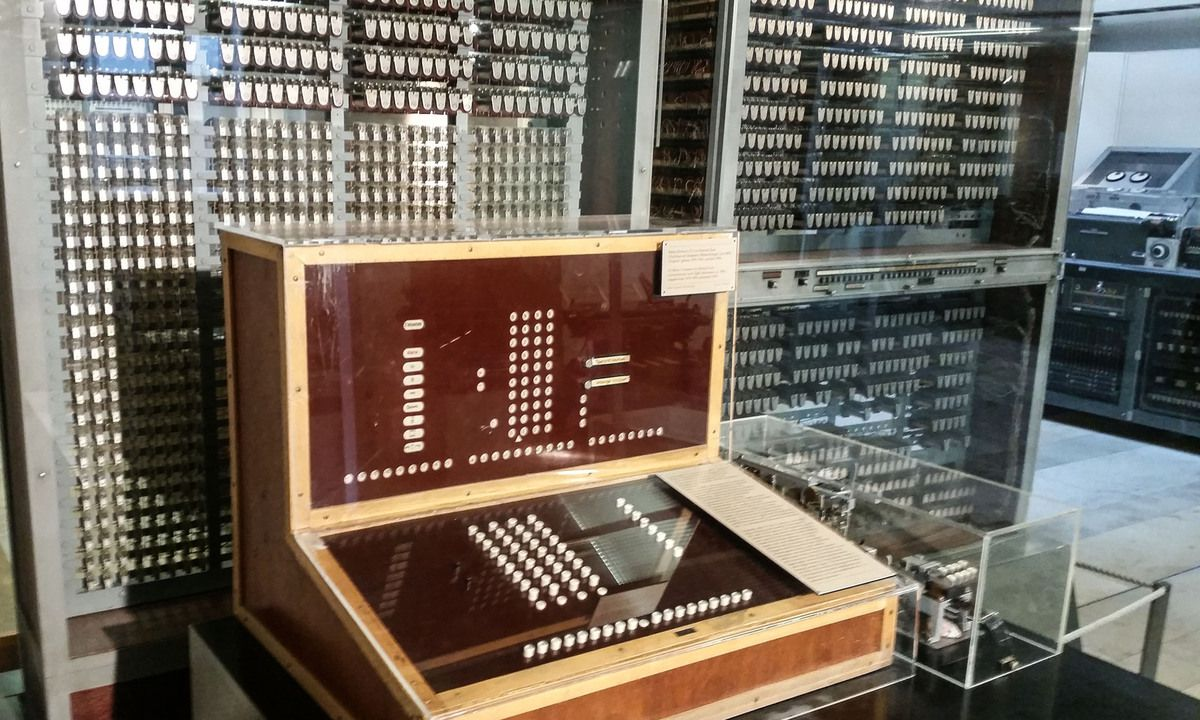
\includegraphics[width=0.5\textwidth]{Images/Z3.jpg}
			\end{center}
	

\end{frame}

\begin{frame}[t]

	\frametitle{Les machines avec des circuits éléctriques : l'ENIAC}
	
	\begin{itemize}
		\item Crée en 1946 et devient le premier ordinateur avec aucune pièce mécanique.
		\item Premier programme écrit par une femme (une première).
		\item Cette machine sera utilisé pour créer la bombe H.
	\end{itemize}
	
			\begin{center}
				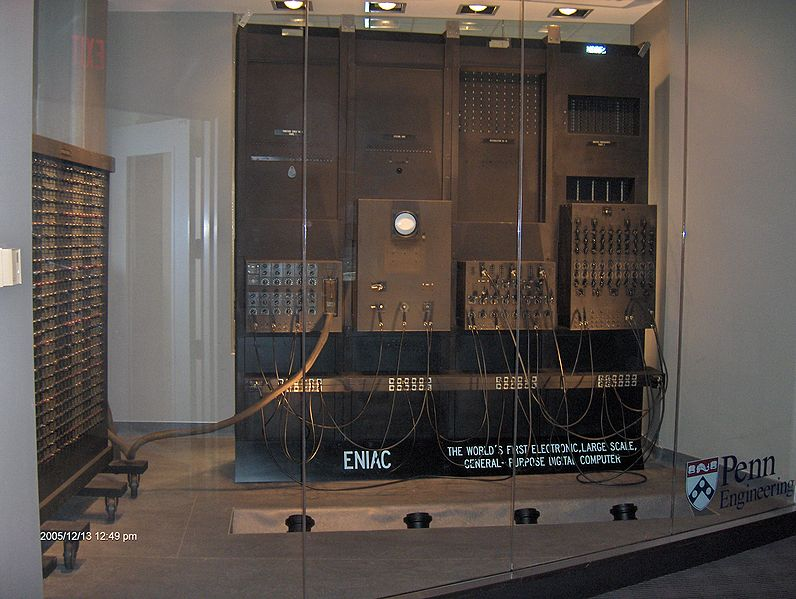
\includegraphics[width=0.5\textwidth]{Images/ENIAC2.jpg}
			\end{center}

\end{frame}

\begin{frame}[t]

	\frametitle{Les premiers ordinateurs personnels}
	
	\begin{itemize}
		\item Création de nouveaux composants informatiques.
		\item Apparition de nouveaux langages de programmations réduisant la taille et le coût des ordinateurs
		\item Création d'un des premiers systèmes d'exploitations UNIX en 1970
		\item Création du 1er micro-processeur par Intel
	\end{itemize}
	
			\begin{flushleft}
				
\includegraphics[width=0.5\textwidth]{Images/UNIX.png}
			\end{flushleft}
			
			\begin{flushright}
				
\includegraphics[width=0.4\textwidth]{Images/Langages.jpg}
			\end{flushright}

			
			
			


\end{frame}

\begin{frame}

	\frametitle{Conclusion}
	
	 Les ordinateurs resteront au cœur de notre vie quotidienne, nous aidant à explorer  de 			 nouveaux horizons et à nous connecter au monde d’une manière que nous ne pouvions imaginer 	     auparavant. On peut conclure que c'est une histoire intéressante marquée par des avancées technologiques extraordinaires.

\end{frame}



\end{document}
